<<<<<<< HEAD
% Folien f�r die Poster-Session VAR2021
\documentclass[aspectratio=169]{beamer}
=======
% Folien f�r die Poster-Session VAR2021
\documentclass{beamer}
>>>>>>> 81430978c5bc12338bc5b87d5b2dc5b53be397ec
% Funktion f�r Footer/Header in den Folien
\newcommand{\lectureName}{Visual Raytrace}
% Titel der Folie
\title{\lectureName}
\author{Manfred Brill, Benedict S�rota}
\institute{University of Applied Sciences Kaiserslautern}
\date[]{}
%
% Variablen wie Semester ...
%
\newcommand{\theSemester}{September 2021}
% Standardverzeichnis f�r das Basis-Verzeichnis der Bilder
%
\newcommand{\imagePath}{../figures}
%
% Name der Bilddatei, die auf die Fragefolie kommen soll
\newcommand{\questionImage}{../figures/vorgang}

\input{slidesheader}
\title{Visual$\:$Raytrace}
\subtitle{VAR 2021 --- Poster Session}
%
%
\subject{Informatik -- Masterstudiengang}
\keywords{Informatik, Masterstudiengang, Master of Science, Hochschule Kaiserslautern, Fachbereich Informatik und Mikrosystemtechnik}
%
\hypersetup{
pdfauthor = {Manfred Brill, Benedict Särota},
pdfsubject = {Poster Visual Raytrace VAR2021},
pdftitle = {MasterstPoster Visual Raytrace VAR2021},
pdfkeywords = {Immersive Learning, Computer Graphics, Raytracing, VR, XR, University of Applied Sciences Kaiserslautern, Computer Science},
pdfpagelayout = SinglePage,
pdfpagemode = UseThumbs,
pdfdisplaydoctitle = true
}

%
\setboolean{solutions}{true}
% Nur Folien: die n�chste Zeile kommentieren!
\setbeameroption{show notes}
<<<<<<< HEAD
% Die n�chste Zeile dekommentieren f�r handouts!
\pgfpagesuselayout{2 on 1}[a4paper, border shrink=5mm]
=======
% Die n�chste Zeile dekommentieren f�r handouts!
%\pgfpagesuselayout{2 on 1}[a4paper, border shrink=5mm]
>>>>>>> 81430978c5bc12338bc5b87d5b2dc5b53be397ec
%
\begin{document}
\begin{frame}
  \titlepage
  \begin{center}
   \includegraphics[width = 5.0cm]{\imagePath/vorgang}
  \end{center}
\end{frame}

\note{
\noteshead{Information}

\begin{itemize}
\item Introduction of presenter
\item Introduction of university / laboratories
\item Introduction of specific project / content of presentation
\end{itemize}

Welcome to my presentation. My name is Benedict Särota and I'm a student, currently finising my masters degree in computer science. Today I will be presenting our virtual reality application "VisualRaytrace" that was developed by me in the Virtual and Augmented Reality Lab, University of Applied Sciences Kaiserslauten at the campus Zweibruecken

}




%\section{Motivation}
%\note{
%\noteshead{Notes}

%Hier k�nnen wir Notizen schreiben, die wir in den Handouts auch ausdrucken k�nnen!

%Als erster Schritt wurden einfach die Bilder und Texte aus dem Poster �bernommen.
%F�r Folien, die nur eine �berschrift und ein Bild verwenden gibt es in slidesheader.tex
%die Funktion \lstinline$\\imageslide$. Erstes Argument ist der Titel, dann die Angabe der Breite (am Besten
%in Prozent der Textbreite) und den Pfad f�r das Bild (relativ zum Inhalt
%der Variablen \lstinline$\\imagePath$.
%}

%\note{
%\noteshead{Textblock}

%Die folgende Folie verwendet den Textblock aus dem Poster oben rechts!
%}

\begin{frame}{Immersive Learning}
\begin{block}{Raytracing}
   \begin{itemize}
   \item Raytracing is one of the major topics in computer graphics classes.
   \item Students have to implement their own version of a working raytracer.
   \item To implement a raytracer students need to understand the basic concepts of computer graphics
   like coordinate systems, camera, lighting or reflection.
   \item Key for the successful implementation of a raytracer by the students: develop a high spatial imagination.
   \item The immersive learning application \textbf{Visual$\:$Raytrace} supports the transfer from 3D space
   to a programming language and deepens the understanding of the basic concepts of a raytracer.
   \end{itemize}
\end{block}
\end{frame}

\note{
\noteshead{Immersive Learning}

<<<<<<< HEAD
Mit \lstinline$\\section$ wird links oben die �berschrift eingestellt (kann man auch leer lassen.
=======
Raytracing is a popular entry level application for computer graphics classes. Using this technology, basic concepts of computer graphics like coordinate systems, cameras or reflection models can be taught, implemented by the students and observed in self-implementation exercises. In practice, this process from the viewpoint of the student consists of application of raw math functions and programming code, compiling the program and receiving a 2D image as output.
>>>>>>> 81430978c5bc12338bc5b87d5b2dc5b53be397ec

}

\section{Whitted Raytracing}
\imageslide{Whitted Raytracing}{0.7\textwidth}{whitted02}

\note{
\noteshead{Raytracing}

\begin{itemize}
\item Introduce raytracing concept
\item Reference picture (Whitted)
\item Illustrate learning process from the perspective of the student
\end{itemize}

Picture: J. Turner Whitted

}

\section{Visual$\:$Raytrace}
\begin{frame}{VisualRaytrace}
\begin{block}{VisualRaytrace}
\begin{itemize}
\item Unity application using HTC Vive Input Utility
\item Raytracing process can be controlled and examined
\item 3D representations of the raytracer embedded into the scene
\end{itemize}
\end{block}

\begin{center}
\includegraphics[width=0.9\textwidth]{../figures/vorgang}
\end{center}

\end{frame}

\note{
\noteshead{Visual$\:$Raytrace}

\begin{itemize}
\item Introduce VisualRaytrace application
\item Mention technical dependencies
\end{itemize}

To test this concept, we implemented the virtual reality application VisualRaytrace. Using the Unity engine and the HTC Vive Input Utility extension, we constructed a walkable area in virtual 3D space that allows the user to watch and control the raytracing process.
Traditional components of a raytracer are represented in the scene. For example, a big white eyeball with a black iris represents the eye or camera, the place from which the rays originate from.

}


\imageslide{Raytracer in a Virtual Environment}{0.9\textwidth}{duringProcess}

\note{
 \noteshead{Raytracer in a virtual environment}

\begin{itemize}
\item Describe raytracer elements in scene
\item Explain process
\end{itemize}

Here we see the main scene of our application. The eye looks through the viewport at a designated target area. Rays are shot through each pixel before hitting different elements of the target area.


}


\imageslide{Virtual Framebuffer and a Virtual Ray}{0.9\textwidth}{duringProcessEyeView}

\note{
 \noteshead{Virtual Framebuffer and Virtual Ray}

	\begin{itemize}
	\item Explain virtual framebuffer, viewport
	\item Explain virtual ray
	\end{itemize}

Let's take the perspective of the eye. The eye shoots pink rays through single pixels of the ingame viewport. Based on the objects hit, the pixel color is set on the texture covering the viewport. This process is repeated until all pixels have been computed and the raytracing has finished, unless the user decides to pause or stop the process using ingame buttons.


}


\imageslide{Ray-Sphere Intersection}{0.9\textwidth}{duringProcessHitObjects}

\note{
 \noteshead{Ray-Sphere Intersection}

	\begin{itemize}
	\item Explain target area
	\item Explain different reflection models, materials
	\end{itemize}

Located behind the viewport is the target area of the raytracer. We see a handful of preset sphere objects with different colors and reflection models. Solid color spheres provide no reflections and simply return their color to the raytracer. Metal spheres do reflect incoming rays, resulting in a mirror like texture in the final image. On the right between the green and blue spheres we have a dielectric sphere, emulating a glass like material with additional internal refraction. The raytracer will hit objects in the area and, depending on the color and reflection model of the assigned object material, reflect or refract until computation of the final pixel color has finished. 


}


\imageslide{Interactive scene definition}{0.9\textwidth}{sphereCreating}

\note{
 \noteshead{Interactive scene definifion}

	\begin{itemize}
	\item Explain creation of additional spheres
	\item Explain swapping sphere materials
	\end{itemize}

Besided merley observing the raytracing process, the user can also interact with the scene in different ways. Additional spheres can be created, infused with one of three reflection models and dropped in the target area of the rays. This allows for custom images to be created using the raytracer. 


}

\imageslide{Settings for the Raytracer}{0.9\textwidth}{settings}

\note{
 \noteshead{Settings for the raytracer}

	\begin{itemize}
	\item Explain settings wall
	\item Explain categories, operations
	\end{itemize}

These images can be extracted from the application and used in further applications by the user. A wall-based settings menu was added to the scene to call on these operations or change properties. Currently, only the raytracers sampling technique and material parameters can be modified. 

}


\section{Software Development}
\imageslide{Unity and C\#}{0.9\textwidth}{unityIDE}

\section{Future development}
\begin{frame}{Future development}
\begin{block}{Next steps...}
\begin{itemize}
\item Standalone version of the raytracer component of the application
\item Scene transition into the target area itself to display further information 
\end{itemize}
\end{block}
\end{frame}

\note{
\noteshead{Next steps...}

\begin{itemize}
\item Standalone library raytracer
\item Second scene of raytracer target area
\end{itemize}

Currently we are developing the raytracer as a standalone library component. This should allow for the application code to be handed out to future students without revealing raytracer code itself. We could even try to use other third party raytracers in our application.

For the application itself we plan to add a second scene, in which the user can enter the raytracer target area itself and be able to more clearly examine the reflections between spheres up close. 

}

\begin{frame}{Future development}
\begin{block}{Future work}
\begin{itemize}
\item Evaluation of the application on campus
\item OpenXR- and WebXR based versions
\end{itemize}
\end{block}

\begin{center}
\includegraphics[width=7cm]{../figures/logos/openXR}
\includegraphics[width=8cm]{../figures/logos/webXR}
\end{center}
\end{frame}

\note{
\noteshead{Future development}

\begin{itemize}
\item Evaluation of the application
\item OpenXR and WebXR versions
\end{itemize}

Further out in the future, we are planning to evaluate this application in a computer graphics class on our campus, once the current pandemic situation improves.

We would also like to base future version of this application on the OpenXR and WebXR frameworks, to allow for the application to run on as many platforms as possible.

}

\questionsEnglish[0.9\textwidth]

\end{document}
